\documentclass{article}
\usepackage{graphicx}
\usepackage[margin=1.5cm]{geometry}
\usepackage{amsmath}

\begin{document}
\twocolumn

\title{Monday Warm Up: Unit 3, Magnetic Forces and Fields}
\author{Prof. Jordan C. Hanson}

\maketitle

\section{Memory Bank}

\begin{itemize}
\item $\vec{F} = q\vec{v} \times \vec{B}$ ... The Lorentz force, one version.
\item $\vec{F} = i\vec{L} \times \vec{B}$ ... The Lorentz force, another version.
\item $\vec{\tau} = \vec{r} \times \vec{F}$ ... Definition of torque.
\item $\vec{\tau} = \vec{\mu} \times \vec{B}$ ... Torque on a current carrying loop in a uniform B-field.
\item $\vec{\mu} = NI\vec{A}$ ... Definition of the magnetic moment.
\item $\vec{B} = \mu_0 I/(2\pi r)\hat{\phi}$ ... B-field created by a straight segment of wire, Amp\`{e}re's Law.
\end{itemize}

\section{Torque, revisited}

\begin{enumerate}
\item Suppose we apply a force $\vec{F} = 10\hat{j}$ N (upward) on the end of a 10 cm wrench it as \textit{loosens} a bolt at the origin.  The bolt is to the left of the wrench.  What is the magnitude \textit{and direction} of the torque? \\ \vspace{1cm}
\end{enumerate}

\section{The Electric Motor}

\begin{enumerate}
\item Let us derive the maximum torque for an electric motor like the one shown in Fig. \ref{fig:lorentz}.  The magnetic moment of a loop of current is $\vec{\mu} = NI\vec{A}$, where $N$ is the number of turns, $I$ is the current, and $\vec{A}$ is the area vector. (a) Based on Fig. \ref{fig:lorentz} (left), show that the torque $\vec{\tau}$ on the current loop is $\vec{\mu} \times \vec{B}$. (b) Given what you know about the cross-product, what is the maximum magnitude of $\vec{\tau}$? \\ \vspace{5cm}
\item Consider Fig. \ref{fig:lorentz}, in which a DC electric motor is depicted inside a 0.05 T B-field.  Suppose the area of the loop is $10^{-2}$ m$^{2}$, the voltage in the circuit is 24 V, and the circuit resistance is 50 $\Omega$.  Also assume that there is just one loop of wire in the rotor.  What is the \textit{maximum torque} the system could achieve? \\ \vspace{3cm}
\item What would the maximum torque be if there were $N = 100$ turns of wire? \\ \vspace{2cm}
\end{enumerate}

\begin{figure}
\centering
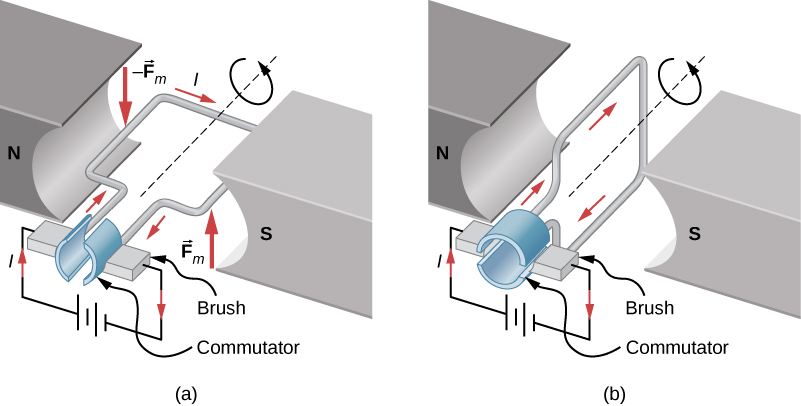
\includegraphics[width=0.55\textwidth]{commute.jpeg}
\caption{\label{fig:lorentz} An illustration of how a power generator works.  This version uses DC current and a commutator.}
\end{figure}

\section{Amp\`{e}re's Law}

\begin{enumerate}
\item What is the magnitude of the B-field created by a 1 A current within a wire, 1 cm away from the wire?  How does this compare to the B-field of the Earth?
\end{enumerate}

\end{document}
